

% ================================
% Random Vectors in High Dimension
% ================================
\begin{figure}[H]
\centering
\begin{tikzpicture}[scale=2.0]

% Draw Square 
\draw[] (0, 0) -- (0, 2) -- (2, 2) -- (2, 0) -- (0, 0);
\draw[dashed] (0.5, 0.5) -- (0.5, 2.5) -- (2.5, 2.5) -- (2.5, 0.5) -- (0.5, 0.5);
\draw[] (2, 2) -- (2.5, 2.5);
\draw[dashed] (0, 0) -- (0.5, 0.5);
\draw[] (2, 0) -- (2.5, 0.5);
\draw[] (0, 2) -- (0.5, 2.5);

\draw[] (0, 0) -- (0, 1) -- (1, 1) -- (1, 0) -- (0, 0);
\draw[dashed] (0.25, 0.25) -- (0.25, 1.25) -- (1.25, 1.25) -- (1.25, 0.25) -- (0.25, 0.25);
\draw[dashed] (1, 1) -- (1.25, 1.25);
\draw[dashed] (0, 0) -- (0.25, 0.25);
\draw[dashed] (1, 0) -- (1.25, 0.25);
\draw[dashed] (0, 1) -- (0.25, 1.25);

\draw[] (0.9, -0.1) -- (1.1, 0.1) node[at start, below] {1};
\draw[] (1.9, -0.1) -- (2.1, 0.1) node[at start, below] {2};
\end{tikzpicture}
\end{figure}


\section{Random Vectors in High Dimensions}
So far, we have covered numerous probability bounds on individual random variables, as well as sums of random variables. Now, we will turn our attention towards random vectors. The driving motivation of extending our theory to random vectors in high dimension is evident based on the typical problems faced in data science. Unlike problems in the past where an outcome could be well estimated with a few covariates, problems in the 21st century must be estimated with thousands of covariates. 

Unfortunately, due to the high dimensionality of today's problems, classical tools in statistics become infeasible to use -- this is dubbed the \textit{curse of dimensionality}. To illustrate why classical tools become infeasible is 



\subsection{Concentration of the Norm}

% =======================================
% Illustration: Concentration of the Norm
% =======================================
\begin{figure}[H]
\centering
\begin{tikzpicture}

    % Draw Grid
    \draw[very thin, gray!40!white] (-0.5, -0.5) grid (4.9, 4.9); % Grid 
    \draw[thick, ->] (-0.5, 0) -- (5, 0) node[anchor=west] {$x$};
    \draw[thick, ->] (0, -0.5) -- (0, 5) node[anchor=south] {$y$};
    
    \draw[very thick, ->, red] (0, 0) -- (3.5, 0) node[anchor=north] {$X$};
    \draw[very thick, ->, blue] (0, 0) -- (0, 2.5) node[anchor=east] {$Y$};
    \draw[very thick, ->] (0, 0) -- (3.5, 2.5) node[anchor=south] {$\left[ \begin{matrix} \textcolor{red}{X} \\ \textcolor{blue}{Y} \end{matrix} \right]$};
    
    \draw[thin, dashed, red] (3.5, 0) -- (3.5, 2.5); 
    \draw[thin, dashed, blue] (0, 2.5) -- (3.5, 2.5); 
    
    % Label Norm
    \draw[decorate, decoration={brace, amplitude=15pt}] (0, 0) -- (3.5, 2.5) node[anchor=south, midway, xshift=-0.3cm, yshift=0.35cm] {$\|X\|_2$};
\end{tikzpicture}
\caption{Curse of Dimensionality}
\end{figure}


% =======
% Theorem: Concentration of Norm
% =======
\begin{remark}[Expected Length of $n$-Dimensional Vector]
Suppose we have an $n$-dimensional vector $X = (X_1, ..., X_n). $ Suppose further that each $X_i$ has mean 0, and variance 1. In order to find the squared norm of $X$, we have
\begin{align*}
    \Expect{\|X\|^2_2} &= \Expect{\sum_{i=1}^{n} X_i^2} && \text{defn. norm} \\ 
    &= \sum_{i=1}^{n} \Expect{X_i^2} && \text{since $X_i$ independent.} \\ 
    &= \sum_{i=1}^{n} 1 && \text{$\Expect{X_i} = 0 \implies Var(X_i) = \Expect{X_i^2} = 1$} \\ 
    &= n
\end{align*}
Therefore, the expected squared euclidean norm of $X$ is $n$, or in other words, the norm of $X$ should be around $\sqrt{n}.$ Although the expected norm is $\sqrt{n}$, we will now turn our attention towards the question of how close the vector will be to its norm. 
\end{remark}

% Drawing Sphere
\begin{figure}[H]
\centering
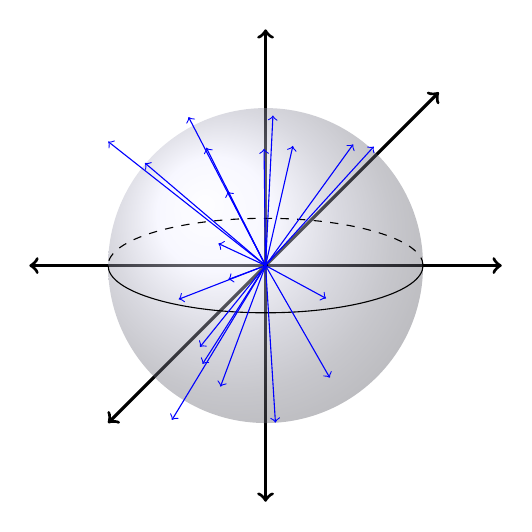
\begin{tikzpicture}

    % Draw Grid
    \draw[very thick, <->] (0,-3) -- (0, 3);
    \draw[very thick, <->] (-3,0) -- (3, 0);
    \draw[very thick, <->] (-2, -2) -- (2.2, 2.2);

    % Draw Sphere
    \shade[ball color = blue!10, opacity = 0.4] (0,0) circle (2cm); % Shade Sphere
    \draw (-2,0) arc (180:360:2 and 0.6);                           % Draw Front Circumference
    \draw[dashed] (2,0) arc (0:180:2 and 0.6);                      % Draw Back Circumference
    \fill[fill=black] (0,0) circle (1pt);                           % Draw Center
%  \draw[dashed] (0,0 ) -- node[above]{$r$} (2,0);                 % Draw Radius
  
    % Draw Random Vectors
    \foreach \i in {1, ..., 20}{
      \draw[->, blue] (0, 0) -- (2*rand, 2*rand);
    }
\end{tikzpicture}
\end{figure}



